\section{Metsandus}
Metsad omavad olulist rolli nii ühiskonna igapäevaelus kui ka planeedi heaolus.
Alates mööblis kasutatavast puidust kuni paberini, millele kirjutame. Lisaks neile
nähtavatele toodetele sisaldavad paljud ravimid, kosmeetika ja pesuvahendid
metsadest saadud kõrvalsaadusi. Rohkem kui 1,6 miljardit inimest sõltub
metsadest toidu ja kütuse saamisest ning umbes 70 miljonit, sealhulgas paljud
põlisrahvad, peavad metsi oma koduks \cite{karsentyUnderlyingCausesRapid2003}. 
Metsad varustavad meid hapnikuga, pakuvad
varjualust, töökohti, puhast vett ja toitu, olles seega inimkonna ellujäämiseks
hädavajalikud. Kuna nii paljude inimeste elu sõltub metsadest, on metsade saatus
otseselt seotud ka meie endi tulevikuga. \cite{WWFImportanceForests}

\section{Copernicus ja EstHub}
Eesti metsade kaugseires on oluline roll Copernicuse programmil ja EstHubi keskusel. Copernicus on üks osa Euroopa kosmoseprogrammist (EUS), mis tegeleb planeedi jälgimisega. Copernicus programmi raames, lisaks maapealse info kogumisele, on loodud mitmeid satelliite, mis koguvad informatsiooni kosmosest. See info on kõigile kättesaadav tasuta. Selle programmiga seotud satelliite kutsutakse \textbf{Sentineliks}. \cite{CopernicusCopernicus}


EstHub on Eesti riiklik satelliitandmete keskus, mis kogub ja integreerib
mitmekesiseid georuumilisi andmeid automatiseeritud protsesside kaudu.
Andmekogumine hõlmab kõrge resolutsiooniga satelliitkaadrite allalaadimist ja
standardiseerimist erinevatest allikatest. EstHubi eesmärk on koguda kokku satelliidi andmed mis katavad Eesti territooriumi. \cite{maa-ametNationalSatelliteData}

\begin{figure}[H]
    \centering
    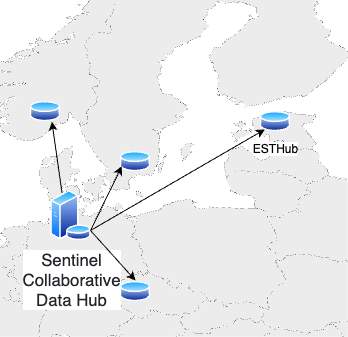
\includegraphics[width=.3\textwidth]{figures/datahubEU.drawio.png}
    \caption{Sateliidi andmete liikumine andmekeskuste vahel}
    \label{fig:esthubliiklus}
\end{figure}


\subsection{Sentinel}
Kaugseire valdkonnas on vastavalt vajadusele kasutusel erinevatelt satelliitidelt pärinevad andmed. Sentinel-1 on radaripõhine satelliit, mis võimaldab jälgida maapinna vajumist,
struktuuride kahjustusi ning looduskatastroofe nagu maavärinad ja maalihked. Samuti on
see ideaalne mere- ja Arktika seireks, sealhulgas laevade jälgimiseks ning
naftareostuse tuvastamiseks. \cite{S1Applications}

Sentinel-2 missioon koosneb kahest identsest satelliidist, Sentinel-2B
(käivitatud 2017) ja Sentinel-2C (käivitatud 2024), mis töötavad koos, et
pakkuda kõrge eraldusvõimega multispektraalseid pilte Maa pindadest,
rannikualadest ja siseveekogudest iga viie päeva järel. Need andmed toetavad
rakendusi põllumajanduses, metsanduses ja maakatte klassifitseerimisel. \cite{S2Applications}

Sentinel-3 on Euroopa Maa seire satelliitmissioon, mille eesmärk on mõõta
merepinna topograafiat, mere ja maa pinnatemperatuure ning ookeani ja maa
pinnavärvi suure täpsusega. Neid andmeid kasutatakse ookeani prognoosisüsteemides,
keskkonnaseires ja kliimaseires. \cite{S3Mission}

Sentinel-5P on esimene Copernicuse missioon, mis on pühendatud atmosfääri
seirele. See kannab tipptasemel \textbf{Tropomi} instrumenti, mis kaardistab mitmeid
gaase nagu lämmastikdioksiid, osoon, formaldehüüd, vääveldioksiid, metaan,
vingugaas ja aerosoolid - kõik need mõjutavad meie hingatavat õhku, tervist ja
kliimat. \cite{S5PApplications}
\subsection{Lainepikkuste spekter}
Spektriribad on satelliitandmete analüüsimisel üliolulised, sest need
võimaldavad eristada maapinna erinevaid omadusi, lähtudes elektromagnetilise
spektri konkreetsetest lainepikkustest. Näiteks Sentinel-2 MSI instrumendi 13
spektririba hõlmavad nähtavat valgust, lähedast infrapunat ja lühilaine
infrapunat, võimaldades detailset maastiku klassifitseerimist, sealhulgas
metsade, veekogude ja muu loodusliku keskkonna eristamist. Iga ribaga seondub
kindel lainepikkuse vahemik, mida spetsiifiliste filtrite abil eraldatakse \cite{S2Mission}.
Ülevaate Sentinel-2 spektriribadest saab Tabelist \ref{tab:s2bands}.
\bigskip

\begin{table}
\caption{Sentinel-2 MSI spektriribad ja nende kasutusvaldkonnad \cite{S2Mission}.}
\label{tab:s2bands}
\begin{longtable}{p{1cm}p{1.6cm}p{1.6cm}p{9cm}}
    \hline
    Riba & Resolutsioon & Keskmine lainepikkus & Kasutus                          \\ 
    \hline
    B01  & 60 $m/px$      & 443 $nm$ & Ultrasinine (aerosool)           \\
    B02  & 10 $m/px$      & 490 $nm$ & Sinine                           \\
    B03  & 10 $m/px$      & 560 $nm$ & Roheline                         \\
    B04  & 10 $m/px$      & 665 $nm$ & Punane                           \\
    B05  & 20 $m/px$      & 705 $nm$ & Lähiinfrapuna (vegetatsiooni klassifitseerimine) \\
    B06  & 20 $m/px$      & 740 $nm$ & Lähiinfrapuna (vegetatsiooni klassifitseerimine) \\
    B07  & 20 $m/px$      & 783 $nm$ & Lähiinfrapuna (vegetatsiooni klassifitseerimine) \\
    B08  & 10 $m/px$      & 842 $nm$ & Lähiinfrapunariba (rannajoonte ja biomassisisalduse kaardistamiseks) \\
    B8A  & 20 $m/px$      & 865 $nm$ & Lähiinfrapuna  \\
    B09  & 60 $m/px$      & 940 $nm$ & Keskinfrapuna (veeauru tuvastus)                       \\
    B10  & 60 $m/px$      & 1375 $nm$ & Keskinfrapuna (pilvede tuvastus)                      \\
    B11  & 20 $m/px$      & 1610 $nm$ & Keskinfrapuna       \\
    B12  & 20 $m/px$      & 2190 $nm$ & Keskinfrapuna       \\
%         &              &                    &                              \\
    \hline
\end{longtable}
\end{table}

Ribade kombinerimine võimaldab luua erinevaid indekseid, mis aitavad
eristada erinevaid maapinna omadusi. Näiteks kasutades lähiinfrapunariba B08 saab luua \textbf{NGR}i indeksi, mis põhineb lähi-infrapuna (LIF), rohelise ja punase kanali järjestusel (tähistatakse LRP), kuvab LIF-signaali punases kanalis, rohelise kanal jääb roheliseks ning punane kanal esitatakse sinisena. Selle tulemusel on tervislik taimestik piltidel eredalt punane, kuna rohelised lehed peegeldavad tugevalt lähi-infrapuna spektri osa. Veekogud, mis neelavad nii nähtavat valgust kui ka lähi-infrapuna, ilmuvad tumedana, mullad ja ehituspinnad, mille peegeldus on mõõdukas kõigis kanalites, võtavad omale hallika või kõikuva tooni. Selline komposiit võimaldab metsanduses efektiivselt hinnata taimede seisundit ja kaardistada metsapiire. Ülevaate erinevate spektriribade kombinatsioonide kasutusest leiab Tabelist \ref{tab:NGR_kasutus}.

\begin{table}
\caption{NGR indeksi värvi kasutusjuhend}
\label{tab:NGR_kasutus}
\begin{longtable}{lp{5cm}l}
    \hline
    Objekt & Peegelduse omadused & Kuvatav värv                          \\ 
    \hline
    Tervislik taimestik & Kõrge LIF-peegeldus, mõõdukas roheline, madal punane & Ere punane \\
    Kahjustatud või hõredam taimestik & Madalam LIF-peegeldus & Pruunikas või roosakas \\
    Veekogud & 	Nii nähtav kui lähi-infrapuna valgus neelatakse & Tume sinine kuni must \\
    Paljas muld / linnapinnad & Mõõdukas peegeldus kõigis kanalites & Hallikas, tan või tsüaan\\
    \hline
\end{longtable}
\end{table}

\subsection{Koordinaatsüsteemid ja CRS}
Satelliidilt saadud andmete maapinnaga sidumiseks on vaja kasutatada koordinaatsüsteeme ja
koordinaatide viite süsteeme (CRS).

Koordinaatsüsteem on meetod, mille abil määratletakse ja kirjeldatakse punktide
asukohti maastikul, kasutades koordinaate. Selles kontekstis eristatakse kahte
tüüpi: geograafilised koordinaatsüsteemid, mis kasutavad laiuse ja pikkuse
väärtusi, ning projekteeritud koordinaatsüsteemid, mis teisendavad
geograafilised koordinaadid lameda kaardi koordinaatideks, kasutades
matemaatilisi projektsioone. CRS ehk koordinaatide viite süsteem määratleb
reeglid ja parameetrid, mille alusel need koordinaadid seonduvad reaalse
maastikuga. \cite{8CoordinateReference}

\section{Masinõppe meetodite kasutus kaugseires}
Käsitletava teemaga seotud, kuid teiste piirkondade põhjal loodud, uurimistööde analüüsimisel prooviti välja selgitada, milliseid meetodeid on üldiselt kaugseires kasutatud, sealjuures kas on ehitatud mudeleid nullist või kasutatud
valmis mudeleid. Samuti oli oluliseks eesmärgiks, välja selgitada, kas nendel juhtudel on kasutatud süvaõpet või mitte. Lisaks sooviti teada saada, mis satelliidi andmeid on varasemalt kasutatud ja kas eri lainepikkuste sidumine on andnud paremaid tulemusi.

Ukraina teadlaste poolt koostatud 2021. aastal välja antud artiklis \glqq Deep Learning for Regular Change
Detection in Ukrainian Forest Ecosystem With Sentinel-2\grqq{} kasutati Copernicus Sentinel-2 satelliidi pilte, mis sisaldasid kõrge resolutsiooniga (10 m) värvi- ja spektrikanaleid, sealhulgas NDVI ja NDMI indekseid, võimaldades jälgida metsamuutusi kuni 5-päevaste intervallidega. Andmekogum loodi käsitsi Kharkivi piirkonnas, kasutades mitut järjestikust pilti ja põhjalikku märgistust, et tagada täpne deforestsatsioonipiirkondade kaardistamine. Uurijad rakendasid süvaõppe meetodeid, kasutades mitut U-Neti varianti (näiteks UNet-diff, UNet-CH, UNet2D, UNet3D, Siamese U-Netid ja UNet-LSTM), et hinnata nii ajast sõltuvaid kui ka ühekordseid lähenemisviise. Eraldi rõhutati piltidevahelise erinevuse kasutamise eeliseid, mis parandas segmentatsioonitulemusi ning tõstis Dice ja F1 skoore. Lisaks ilmnesid uuringus olulised nüansid, nagu pilvekatte, hooajaliste muutuste ning geograafiliste lahknevuste mõju, mis nõudsid täiendavat andmete eeltöötlust. Huvitav on, et kuigi kõik mudelid näitasid potentsiaali, saavutavad UNet-diff ja UNet-CH kõige kõrgema täpsuse, pakkudes seeläbi tõenduspõhiseid lahendusi metsakatteta ala muutuste regulaarseks jälgimiseks. \cite{isaienkovDeepLearningRegular2021}

Uus-Meremaal läbi viidud ja 2024. aastal välja antud uurimistöös \glqq Developing a forest description from remote sensing: Insights from
New Zealand\grqq{} kasutati kõrglahutusega lennufotosid ning regionaalseid ALS-andmeid radiata männi metsade täpseks kaardistamiseks Uus-Meremaal. Analüüs tugines sügavõppepõhisel semantilise segmentatsiooni mudelil, mis kasutab DeepLabv3+ arhitektuuri koos ResNext-101 peaahelana (backbone), saavutades IoU väärtused 0,94, täpsuse 0,96 ja meeldetuletuse 0,98. Keeruliseks osutus aga noorte istikute tuvastamine, mille puhul \textit{juvenile} klass (noored istutatud metsapiirkonnad) liideti \textit{radiata} (küpsemad männi alad) klassiga. Lisaks sügavõppemudelile kasutati mitmemuutujalisi regressioonimudeleid metsade keskmise kõrguse, kogumahte ja vanuse hindamiseks, saavutades kõrged R2 väärtused. \cite{pearseDevelopingForestDescription2025}

Kokkuvõtvalt nägin <seda ja seda> ja sellest tulenevalt proovin ka enda lõputöös. 